%begin-include
\section{Software for Ranking of Models of Signaling Networks}
In this section we describe the software we used to perform the ranking
of signaling network models. The first software, SigNetMS, is an 
implementation of the model ranking method presented on 
section~\ref{sec:marginal_likelihood_method}, which estimates the 
marginal likelihood of the data being reproduced by a model.  The second 
software, ABC-SysBio implements the method based on the approximate 
Bayesian Computation, presented on section~\ref{sec:abc_method}.

\subsection{SigNetMS}
To perform the model ranking using an estimate of the marginal 
likelihood, we created the software SigNetMS, which is an acronym of 
{\bf Sig}naling {\bf Net}work {\bf M}odel {\bf S}election. This software
was implemented in Python and it is a free software, under the \emph{GNU 
General Public License}, and available on
\href{https://github.com/gustavoem/SigNetMS}{GitHub}. The SigNetMS 
software can read and parse files containing models of signaling network 
represented in the Systems Biology Markup Language (SBML) format and 
then construct the respective system of differential equations according 
to the chemical species and interactions defined on the file. The 
experiments observations and prior distributions of parameters are 
defined by the user with Extensible Markup Language (XML) files. Four 
other parameters are necessary to run SigNetMS, all of them related to 
the sampling of the power posteriors. 

The method we used to sample each of the power posterior distributions
is the one we presented on section~\ref{sec:power_posteriors_sampling}.
The four parameters related to the sampling determine the size of all
sampling  performed and also the adaptive behaviour of one of the 
Metropolis-Hastings algorithm used. The first parameter defines the 
number of iterations of the first sampling algorithm. This algorithm is 
adaptive because, after a fixed number of iterations, the covariance of 
the jump distribution is updated according to the acceptance rate of 
proposed points; this fixed number of iterations is the second sampling 
parameter. Finally, the third and fourth parameter determine the size of
the second and third sampling steps respectively.

To implement the method we still have to define the proposal 
distributions. Since the proposed model parameters cannot have 
nonpositive values (because they are reaction rate constants), the 
proposal distribution should have a probability density function that 
has value zero for nonpositive numbers. Moreover, its desired, through 
the sampling steps, to control the mean and variance of the proposal 
distributions. For all of the three steps, if the current point of the
chain is $\theta$, then the jump distribution should have mean close
to $\theta$. Also, in the first step, the covariance matrix  of the 
proposal distribution should be proportional to the covariance of 
the prior distribution of parameters. Then, for the two final steps, the 
covariance matrix of the jump distribution should be proportional to an
estimate $\hat{C}$ of the covariance of the parameters, calculated with 
the accepted points of the chain.

In our first attempt, we used multivariate lognormal distributions for 
all the sampling steps. If $X$ is a $MultivariateNormal (\mu, \Sigma)$, 
then $Y = e^{X}$ is $MultivariateLognormal (\mu, \Sigma)$. However, we 
found out that for some combinations of $\theta$ and $\hat{C}$, there 
is no combination of parameters $(\mu, \Sigma)$ such that $Y \propto 
MultivariateLognormal (\mu, \Sigma)$ with $\expectation[Y] = \theta$ and
$var(Y) = \hat{C}$. Then the solution we proposed is to use a truncated 
normal distribution for which only positive numbers have positive 
probability. We can generate a truncated normal random variable, 
$Y \propto TruncatedNormal (\mu, \Sigma)$ by 
repeatedly generating a normal random variable, $X \propto Normal(\mu, 
\Sigma)$ until $X$ is positive. However, this approach has the drawback 
that  $\expectation[Y]$ is usually greater than $\mu$, implying on a 
biased run of Metropolis-Hastings.
{\color{blue} Maybe we should state here that we can't calculate pdf of
the truncated normal distribution?}

The SigNetMS program also has an optional argument that allows the user
to get a verbose run, showing all proposed parameters for each 
temperature as well as the accepted parameters used to estimate the 
logarithm of the marginal likelihood. 

%-> implemented in Python
%-> implements the ABC-SMC method we explained earlier
%-> also reads models in SBML format
\section{ABC-SysBio}
ABC-SysBio is a Python software that implements the Approximate Bayesian
Computation Sequential Monte Carlo (ABC SMC) method~\cite{Liepe2010}. 
This software, similarly to SigNetMS, also takes as input SBML models as 
well as prior distribution of parameters and experimental data. As the 
output, the software returns, for each candidate model, an estimate of 
the probability of that model reproducing the experimental data. The 
source code of the method is available on 
\href{https://sourceforge.net/projects/abc-sysbio/files/}{SourceForge}.

\section{Model Selection Experiments}
The experiments we performed to test both methods consists in taking 
four candidate models and ranking them according to experimental data 
generated by one of them. To generate the simulation data of the 
"correct" model, a set of parameter values, time frames, and a 
measurement based on the concentration of the chemical species is 
chosen; then, a simulation of the model is generated and the artificial 
measurements are produced, with an introduced Gaussian error with mean
zero and standard deviation $0.01$. After that, all information used to
generate data is discarded and the models are ranked based on the 
simulated measurements and prior distributions only.

We performed two experiments, the first is presented 
in~\cite{Vyshemirsky2007} and consists of a common structure in signal 
transduction; the second, created for this project, consists of a 
simpler network, containing a few enzymatic reactions and other first 
order chemical interactions.

\subsection{The First Experiment}
The four candidate models of the first experiment are presented in 
figure~\ref{fig:girolami_models}. The model 1, represented on figure
~\ref{fig:gir_hyp1} is used to generate artificial experimental data
for which all models will be ranked. This network has as components the
degradation of S into dS with reaction rate constant $k_1$; a reversible 
second order reaction \ce{R + S <=> RS} with forward constant rate $k_2$ 
and reverse constant rate of $k_3$; a first order reaction 
\ce{RS -> R_{pp}}; and a Michaelis-Menten (MM) reaction \ce{R_{pp} -> R} 
for which the reaction rate constant and the omitted enzyme 
concentration are combined into one single parameter $V$. Model 2, on 
figure~\ref{fig:gir_hyp2} is a simplification of model 1 in which the
enzymatic reaction of phosphorilation of R is reformulated as a 
MM reaction with enzyme $S$; the other MM reaction, \ce{R_{pp} -> R}, 
now has speed constant $V$ and MM constant $k_3$. Model 3, on figure
\ref{fig:gir_hyp3}, is a simplification of model 2 because it neglects 
the degradation of the chemical species S into dS. The model 4, on 
figure~\ref{fig:gir_hyp4}, is a more complex version of model 1, in 
which the dephosphorylation of R$_{pp}$ is not simplified as a MM 
reaction.

\begin{figure}[H]
  \centering 
  \begin{tabular}{c c}
    \subfigure[]{
    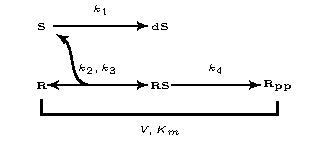
\includegraphics[clip=true,width=.45\linewidth]{experiments/diagrams/bioinformatics_model1.pdf}
    \label{fig:gir_hyp1}}
    &
    \subfigure[]{
    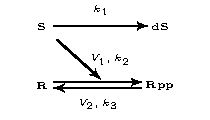
\includegraphics[clip=true,width=.45\linewidth]{experiments/diagrams/bioinformatics_model2.pdf}
    \label{fig:gir_hyp2}} \\
    \subfigure[] {
    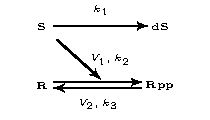
\includegraphics[clip=true,width=.45\linewidth]{experiments/diagrams/bioinformatics_model3.pdf}
    \label{fig:gir_hyp3}}
    &
    \subfigure[] {
    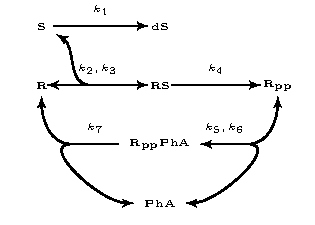
\includegraphics[clip=true,width=.45\linewidth]{experiments/diagrams/bioinformatics_model4.pdf}
    \label{fig:gir_hyp4}}
    \end{tabular}
    \caption{The four models used on the first experiment. The 
    experimental measurement on those models is the concentration of the
    chemical species $R_{pp}$ over time. Model~\ref{fig:gir_hyp1} was
    used to generate artificial experimental data for which those models
    are ranked. Model~\ref{fig:gir_hyp2} is a simplification of the 
    first model in which the phosphorylation of $R$ to $R_{pp}$ was 
    simplified using the Michaelis-Menten kinetics. 
    Model~\ref{fig:gir_hyp4} is a more complex version of the first 
    model. Finally, model~\ref{fig:gir_hyp3} is a very simplified 
    version of the first model, because it neglects the degradation of 
    $S$.}
  \label{fig:girolami_models} 
\end{figure}

The experimental measurement chosen for the hypothesis is the 
concentration of R$_{pp}$ on the time steps: 2s, 5s, 10s, 20s, 40s, 
60s, and 100s. The parameter values chosen for simulation are: 
$k_1 = 0.07$, $k_2 = 0.6$, $k_3 = 0.05$, $k_4 = 0.3$, $V = 0.017$, and
$K_m = 0.3$. The model is then simulated and a Gaussian error with mean
zero and standard deviation $0.01$ is added to the simulation data; this
procedure is repeated three times and hence produces three experimental
observations. Figure~\ref{fig:girolami_simulation} shows one of the 
experimental observations.
\begin{figure}
    \begin{center}
    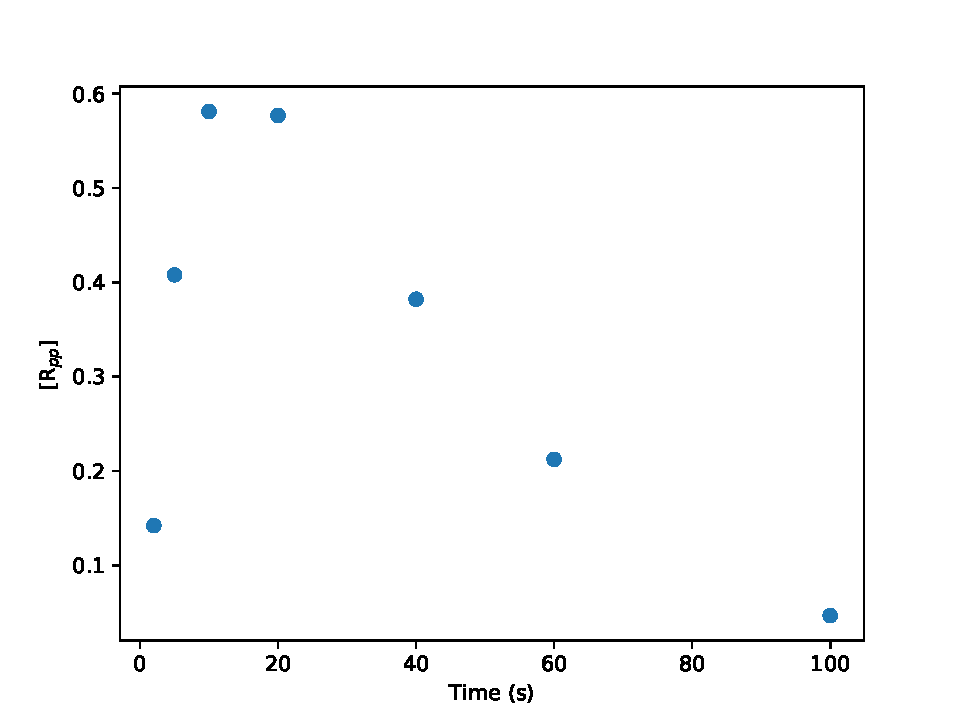
\includegraphics[width=.65\textwidth]{experiments/simulations/girolami_data.pdf}
    \caption{Artificial experimental observation generated with model 1.}
    \label{fig:girolami_simulation}
    \end{center}
\end{figure}


\section{Results}


